\documentclass[crop,tikz]{standalone}

\usepackage[utf8]{inputenc}

% 'crop' is the default for v1.0, before it was 'preview'
%\usetikzlibrary{...}% tikz package already loaded by 'tikz' option

%tikz structures and patterns
\usetikzlibrary{patterns}

%this defines a fill pattern called hexagons
\def\hexagonsize{0.2cm}
\pgfdeclarepatternformonly
  {hexagons}% name
  {\pgfpointorigin}% lower left
  {\pgfpoint{3*\hexagonsize}{0.866025*2*\hexagonsize}}%  upper right
  {\pgfpoint{3*\hexagonsize}{0.866025*2*\hexagonsize}}%  tile size
  {% shape description
   \pgfsetlinewidth{1.2pt}
   \pgftransformshift{\pgfpoint{0mm}{0.866025*\hexagonsize}}
   \pgfpathmoveto{\pgfpoint{0mm}{0mm}}
   \pgfpathlineto{\pgfpoint{0.5*\hexagonsize}{0mm}}
   \pgfpathlineto{\pgfpoint{\hexagonsize}{-0.866025*\hexagonsize}}
   \pgfpathlineto{\pgfpoint{2*\hexagonsize}{-0.866025*\hexagonsize}}
   \pgfpathlineto{\pgfpoint{2.5*\hexagonsize}{0mm}}
   \pgfpathlineto{\pgfpoint{3*\hexagonsize+0.2mm}{0mm}}
   \pgfpathmoveto{\pgfpoint{0.5*\hexagonsize}{0mm}}
   \pgfpathlineto{\pgfpoint{\hexagonsize}{0.866025*\hexagonsize}}
   \pgfpathlineto{\pgfpoint{2*\hexagonsize}{0.866025*\hexagonsize}}
   \pgfpathlineto{\pgfpoint{2.5*\hexagonsize}{0mm}}
   \pgfusepath{stroke}
  } 
  
\begin{document}

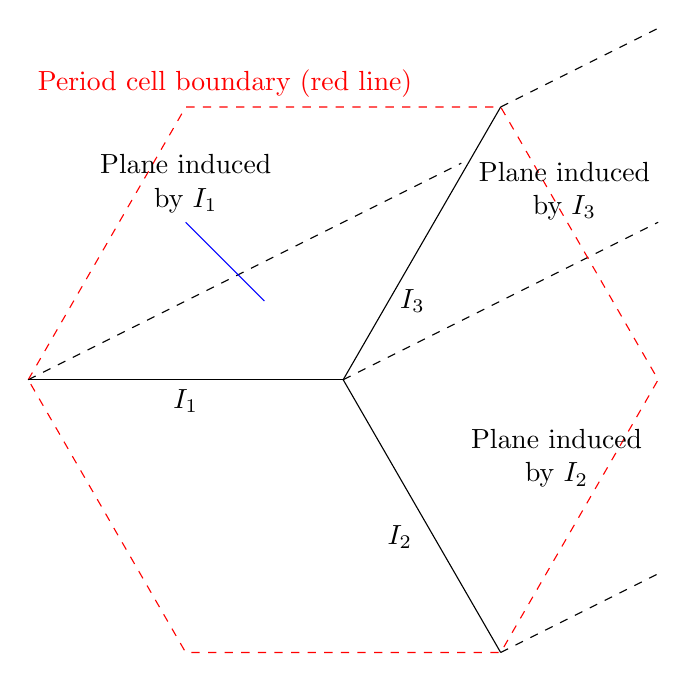
\begin{tikzpicture}

	%x_1,x_2-plane with period cell highlighted
	%\draw[pattern=hexagons] (0,0) rectangle (4,4);	
	
	\begin{scope}[scale=2.0, shift={(0,0)}]
		%induced planes by the singular structure
		\draw[dashed] (2,0) -- (4,1);
		\draw[dashed] (0,0) -- (2.75,1.375);
		\draw[dashed] (3,{sqrt(3)}) -- (4,{sqrt(3)+0.5});
		\draw[dashed] (3,{-sqrt(3)}) -- (4,{0.5-sqrt(3)});
		
		%period cell outline plus crystal lines in the x_1,x_2 plane
		\begin{scope}[scale=1.0, shift={(0,0)}]
			\draw[dashed, red] (0,0) -- (1,{sqrt(3)}) -- (3,{sqrt(3)}) -- (4,0) -- (3,{-sqrt(3)}) -- (1,{-sqrt(3)}) -- cycle;
			\draw (2,0) -- (0,0);
			\draw (2,0) -- (3,{sqrt(3)});
			\draw (2,0) -- (3,{-sqrt(3)});
	\end{scope}
	\node[anchor=south, red] at (1.25,{sqrt(3)}) {Period cell boundary (red line)};	
	
	%labelling for edges and planes
	\node[anchor=north] at (1,0) {$I_1$};
	\node[anchor=south, align=center] at (1,1) {Plane induced  \\ by $I_1$};
	\draw[blue] (1,1) -- (1.5,0.5);
	\node[anchor=east] at (2.5,-1) {$I_2$};
	\node[anchor=west, align=center] at (2.75,-0.5) {Plane induced \\ by $I_2$};
	\node[anchor=west] at (2.3,0.5) {$I_3$};
	\node[anchor=west, align=center] at (2.8,1.2) {Plane induced \\ by $I_3$};
	\end{scope}


\end{tikzpicture}

\end{document}